\section{Wprowadzenie teoretyczne}

\epigraph{There is nothing so practical as a good theory.}{Lewin Kurt}
%\epigraph{Nie ma osobnej ani teorii, ani praktyki inżynierskiej, jest tylko wspólna sztuka inżynierska.}{prof. Jan Oderfeld}

Przygotowując się do projektu o charakterze fizycznym ważnym jest, aby przed rozpoczęciem prac programistycznych dokonać dokładnego przeglądu wiedzy domenowej. Chcąc uzyskać wyniki jakościowe zgodne ze zjawiskami występującymi w rzeczywistości należy zorientować się, czy dla implementowanych zjawisk znane i wykorzystywane są modele fizyczne oraz czy można w sposób w zwięzły zbudować na ich podstawie model matematyczny. Dodatkowo w projekcie o charakterze ogólnym pożądane jest, aby wykorzystane modele były modelami fenomenologicznymi, tj. takimi w których zależności wynikają z podstawowych praw fizyki, a każdemu z parametrów można przypisać pewną interpretację fizyczną. Odrzucając powyższe podejście i opracowując projekt w oparciu o intuicję programisty, mogłoby się okazać, że rezultaty otrzymywane są w sposób nieprzewidywalny, cały projekt posiada jedynie walory estetyczne.\\

Celem tego rozdziału jest przybliżenie wiedzy domenowej, która została wykorzystania podczas realizacji tego projektu. Szczegółowo omówiony został model dynamiki BSP, sterowanie BSP oraz nawigacja. Drugą część rozdziału stanowi teoretyczny opis elementów grafiki komputerowej, wykorzystanych podczas implementacji wizualizacji. Przedstawione zagadnienia zostaną zaprezentowane w sposób umożliwiający ich zrozumienie oraz dalszą implementację, lecz  bez dowodów poprawności. Brak formalności zostanie natomiast zrekompensowany poprzez wskazanie odpowiednich źródeł naukowych.

\subsection{Dynamika lotu BSP}

Przedmiotem zainteresowań dynamiki jest zależność pomiędzy siłami działającymi na analizowany układ a ruchem tego układu.\cite{mw}.  Do opisu dynamiki można skorzystać z różnych narzędzi matematycznych, w zależności od zastosowania oraz własnych preferencji. Najbardziej uniwersalny opis uzyskuje się przez przedstawienie zależności jako układ równań różniczkowych. W publikacjach z zakresu analizy lotu najczęściej można spotkać się właśnie z takim opisem.\cite{energies}\cite{quaterion} Często jednak równania te, ze względu na stopień skomplikowania nie mają analitycznego rozwiązania co rodzi potrzebę efektywnego ich rozwiązywania przy pomocy metod numerycznych. Zbliżonym podejściem posługują się osoby związane z robotyką, który do opisu dynamiki wykorzystują równania stanu, tj. usystematyzowany macierzowy sposób reprezentacji układów równań różniczkowych i algebraicznych. Sprowadzenie równań różniczkowych do wspomnianej formy umożliwia skorzystanie z wielu metod opracowanych właśnie do analizy równań stanu. Warto zasygnalizować, w rozumieniu robotyków BSP stanowi nic innego jak latającego robota mobilnego, których analiza jest często poruszana w tej dziedzinie wiedzy.

\subsubsection{Metody numerycznego rozwiązywania równań różniczkowych}

Metody numeryczne rozwiązywania równań różniczkowych to metody pozwalające na znalezienie przybliżonego rozwiązania tzw. zagadnienia początkowego. Zagadnieniem początkowy nazywamy układ równań różniczkowych wraz ze zbiorem warunków początkowych, pozwalającym na uzyskanie jednoznacznego rozwiązania w funkcji zmiennej niezależnej. Dla symulacji naturalnym wyborem dla zmiennej niezależnej będzie czas \texttt{t}, a warunki początkowe będą związane z początkowymi parametrami BSP (pozycją, orientacją itd.).

\[
	\begin{cases}
		\dot{\bm{y}} \left( t \right)  = \bm{f} \left( t,\bm{y}\right) \\
		\bm{y} \left( t_0 \right) = \bm{y_0}
	\end{cases}
\]

Do rozwiązywania układów równań różniczkowych zwyczajnych (URRZ), bo takie pojawią się w tym projekcie, najczęściej wykorzystuje się numeryczne metody ich całkowania. Przed zastosowaniem każdego z opisanych algorytmów należy jednak równania odpowiednio przygotować i przedstawić je w postaci układu równań różniczkowych zwyczajnych rzędu I. Jest to możliwe dzięki zastosowaniu metody, której wynikiem jest zastąpienie równania różniczkowego \texttt{n}-tego rzędu, układem \texttt{n} równań rzędu pierwszego. Taka zamiana zwiększa jednak liczbę równań i wymaga wprowadzenia zmiennych pomocniczych. Na szczęści w zagadnieniach fizycznych okazuje się często, ze każda ze zmiennych pomocniczych ma interpretację fizyczną i może okazać się użyteczna. po sprowadzeniu układu równań do przedstawionej powyżej formy możliwe jest zastosowanie algorytmu całkowania. Ogólna idea tych metod opiera się na wykorzystaniu obliczonej pochodnej do wykonania małego kroku odpowiadającego przyrostowi czasu. To jak wiele kroków i w jakim punkcie obliczona zostanie pochodna zależy już od konkretnego algorytmu.
Ogólna postać schematu całkowania może zostać przedstawiona jako:

\[
	\bm{y}_{k+1} = \bm{y}_{k} + \bm{F} \left( t_{k-(n-1)}, \bm{y}_{k-(n-1)}, ... t_{k}, \bm{y}_{k},  t_{k+1}, \bm{y}_{k+1}  \right)
\]
gdzie: $\bm{y}_{k}$ oznacza wartość zmiennej zależnej w odpowiadających chwilach $t_{k}$, a~różnice pomiędzy kolejnymi chwilami czasu nazywamy krokiem całkowania $h$.
 

W ogólności dokonuje się podziału metod numerycznego całkowania równań różniczkowych na metody jawne i metody niejawne, metody jednokrokowe (samostartujące) i metody wielokrokowe, a także określa się rząd dokładności i stabilność metody \cite{met_num_szumbi}. Metoda jawne to metody w których funkcja $\bm{F}$ nie zależy od $\bm{y}_{k+1}$. Analogicznie metoda niejawna to taka w której funkcja $\bm{F}$ zależy od $\bm{y}_{k+1}$. Należy zauważyć, że przed zastosowaniem algorytmu niejawnego należy podjąć pewne kroki mające na celu przekształcić funkcję uwikłaną do funkcji prostej. Metody jednokrokowe to metody wykorzystujące tylko aktualną i ew. następną wartość zmiennej zależnej, a więc w ich schemacie $n = 1$. Dla większych wartości $n$ mamy do czynienia z metodami wielokrokowymi. Rząd dokładności jest stopień ostatniej potęgi w szeregu Taylora, któremu odpowiada rozwiązanie uzyskane daną metodą. W praktyce oznacza to jak bardzo długość kroku całkowania wpływa na błąd metody. Im wyższy rząd tym mniejszy błąd metody. Pojęcie stabilności odnosi się natomiast do maksymalnej długości kroku całkowania który nie będzie powodował lawinowego wzrostu błędu metody. Im metoda jest bardziej stabilna, tym dłuższy krok może zostać zastosowany przy całkowaniu równań.\\

W projekcie wykorzystane zostały tylko schematy jawne: metoda Eulera, metoda Heuna, metoda Rungego-Kutty 4 rzędu, a także metody typu predyktor-korektor. Dla metod jawnych możliwe jest opracowanie wspólnego interfejsu. W przypadku metod niejawnych nie byłoby to możliwe ze względu na potrzebę rozwiązania funkcji uwikłanej. \\

\textbf{Jawna metoda Eulera} to najprostszy z algorymów całkowania URRZ. Jest metodą jednokrokową, pierwszego rzędu. Schemat metody całkowania wygląda następująco:
\[
	\bm{y}_{k+1} = \bm{y}_{k} + h \cdot  \bm{f} \left( t_{k}, \bm{y}_{k} \right) 
\]

\textbf{Metoda Heuna} to metodą jednokrokową, drugiego rzędu. Schemat metody całkowania wygląda następująco:
\[
	\begin{aligned}
	k_1 & =  \bm{f} \left( t_{k}, \bm{y}_{k} \right)\\
	k_2 & =  \bm{f} \left( t_{k} + h, \bm{y}_{k} +  h \cdot k_1  \right)\\
	\bm{y}_{k+1} & = \bm{y}_{k} + \frac{h}{2} \cdot  \left( k_1 + k_2 \right)
	\end{aligned}
\]

\textbf{Metody Rungego-Kutty} to rodzina metod jednokrokowych. Najcześciej spotykana jest metoda rzędu czwartego, która jest najbardziej optymalną ze względu na stosunek rzędu i liczby operacji w algorytmie metody.  Schemat metody rzędu 4 wygląda następująco:
\[
	\begin{aligned}
	k_1 & =  \bm{f} \left( t_{k}, \bm{y}_{k} \right)\\
	k_2 & =  \bm{f} \left( t_{k} + \frac{h}{2}, \bm{y}_{k} + \frac{h}{2} \cdot k_1 \right)\\
	k_3 & =  \bm{f} \left( t_{k} + \frac{h}{2}, \bm{y}_{k} + \frac{h}{2} \cdot k_2 \right)\\
	k_2 & =  \bm{f} \left( t_{k} + h, \bm{y}_{k} +  h \cdot k_3  \right)\\
	\bm{y}_{k+1} & = \bm{y}_{k} + \frac{h}{6} \cdot  \left( k_1 + 2 \cdot k_2 + 2 \cdot k_3 +k_4 \right)
	\end{aligned}
\]

\textbf{Metody predyktor-korektor} to grupa jawnych metod, których idea opiera się podzieleniu obliczeń na dwie fazy: fazę predykcji i fazę korekcji. W fazie predykcji jawna metoda wykorzystywana jest do estymacji wartości $\bm{y}_{k+1}$. Następnie w fazie korekty stosuje się schemat niejawny, lecz z wykorzystaniem wartości estymowanej. Sprawia to, że metoda pozostaje jawna, a obszar jej stabilności powiększa się tak jak ma to miejsce w metodach niejawnych. Najczęściej w metodach predyktor-korektor stosuje się jawny schemat Adamsa-Bashforth'a i niejawny schemat Adamsa-Moultona w odpowiadającym rzędzie. Schemat metody rzędu 2 wygląda następująco:
\[
	\begin{aligned}
	\bm{\hat{y}}_{k+1} & = \bm{y}_{k} + 1.5 \cdot h \cdot  \bm{f} \left( t_{k}, \bm{y}_{k} \right) - 0.5 \cdot h \cdot  \bm{f} \left( t_{k-1}, \bm{y}_{k-1} \right)\\
	\bm{y}_{k+1} & = \bm{y}_{k} + \frac{h}{2} \cdot  \left( \bm{f} \left( t_{k} + h, \bm{\hat{y}}_{k+1} \right) +  \bm{f} \left( t_{k}, \bm{y}_{k} \right) \right)
	\end{aligned}
\]

Schemat metody rzędu 4 wygląda następująco:
\[
	\begin{aligned}
	\bm{\hat{y}}_{k+1} & = \bm{y}_{k} + \frac{55}{24} \cdot h \cdot  \bm{f} \left( t_{k}, \bm{y}_{k} \right) - \frac{59}{24} \cdot h \cdot  \bm{f} \left( t_{k-1}, \bm{y}_{k-1} \right)  + \frac{37}{24} \cdot h \cdot  \bm{f} \left( t_{k-2}, \bm{y}_{k-2} \right)  - \frac{9}{24} \cdot h \cdot  \bm{f} \left( t_{k-3}, \bm{y}_{k-3} \right) \\
	\bm{y}_{k+1} & = \bm{y}_{k} +   \frac{9}{24} \cdot h \cdot \bm{f} \left( t_{k} + h, \bm{\hat{y}}_{k+1} \right) + \frac{19}{24} \cdot h \cdot  \bm{f} \left( t_{k}, \bm{y}_{k} \right) - \frac{5}{24} \cdot h \cdot  \bm{f} \left( t_{k-1}, \bm{y}_{k-1} \right)  + \frac{1}{24} \cdot h \cdot  \bm{f} \left( t_{k-2}, \bm{y}_{k-2} \right)
	\end{aligned}
\]

Przedstawione metody są metodami wielokrokowymi, co powoduje ze do swojej pracy wymagają informacji o wartości funkcji prawych stron w poprzednich chwilach czasowych. Powoduje to, że dla zdefiniowanego powyżej zagadnienia początkowego nie pozwalają na policzenie $n-1$ pierwszych kroków całkowania. Rozwiązanie stanowi wykorzystanie algorytmu jednokrokowego do wystartowania metody. Warto również zauważyć, ze obliczenie funkcji prawych stron może być kosztowne obliczeniowo, a dzięki właściwej implementacji można liczbę wywołań znacząco zredukować. W projekcie implementacja metod zakłada użycie bufora cyklicznego do przechowywania wartości funkcji $\bm{f}$ z poprzednich punktów czasowych.

\subsubsection{Równania stanu}

Równania stanu to ujednolicona macierzowa postać zapisuj dynamiki układu. Równania stanu łączą zestaw równań różniczkowych zwyczajnych z równaniami algebraicznymi. W postaci ogólnej liniowej równania stanu prezentują się następująco:
\[
	\begin{cases}
		\dot{\bm{x}} \left(t\right)  = \bm{Ax} \left(t\right)  + \bm{Bu} \left(t\right) \\
		\bm{y} \left(t\right) = \bm{Cx} \left(t\right) + \bm{Du} \left(t\right)
	\end{cases}
\]
gdzie:
\begin{itemize}
\item $\bm{x}$ - wektor stanu układu,
\item $\bm{u}$ - wektor sterowania,
\item $\bm{y}$ - wektor wyjść,
\item $\bm{A}$ - macierz stanu,
\item $\bm{B}$ - macierz wejść,
\item $\bm{C}$ - macierz wyjść,
\item $\bm{D}$ - macierz przenoszenia.
\end{itemize}




\begin{figure}[!h]
   	\centering
      	\includegraphics[width=0.7\textwidth]{state\_eq.png}
      	\caption{Schemat blokowy równań stanu}
      	\label{rnie_stanu}
\end{figure}

Powyższe równania można również przedstawić przy pomocy schematu blokowego przedstawionego na rysunku (\ref{rnie_stanu}).
Intuicyjnie macierz  $\bm{A}$ opisuje swobodną odpowiedź oraz jego zachowanie gdy nie działają na niego żadne wymuszenia. Macierz $\bm{B}$ opisuje w jaki sposób możemy wpływać na układ. Macierz $\bm{C}$ definuje wpływ stanu układu na wyjście. Macierz $\bm{D}$ definiuje jak sterowanie przekłada się bezpośrednio na wyjście, z pominięciem układu. Oprócz usystematyzowanej formy sprowadzenie do równań stanu pozwala w łatwy sposób dokonać analizy dodatkowych własności układu takich jak stabilność, sterowalność i obserwowalność.\\

Znaczącym ograniczeniem przedstawionej postaci jest wymóg opisania układu przy pomocy równań liniowych. Niestety prawa rządzące fizyką rzadko kiedy przyjmują postać liniową. Dowolna nieliniowość powoduje, że równania stanu w formie liniowej przestają być użyteczne. Z tego względu powszechnie stosowana jest forma nieliniowa równań stanu, która prezentuje się następująco:
\[
	\begin{cases}
		\dot{\bm{x}} \left(t\right)  =  \bm{f}  \left( t, \bm{x} \left(t\right)  , \bm{u} \left(t\right) \right) \\
		\bm{y} \left(t\right) = \bm{g}  \left( t, \bm{x} \left(t\right) , \bm{u} \left(t\right) \right)
	\end{cases}
\]

Obie przedstawione postaci są ze sobą ściśle powiązane. Postać liniową można bez starty ogólności sprowadzić do postaci nieliniowej, a poprzez linearyzację w otoczeniu przyjętego punktu równowagi można sprowadzić postać nieliniową do jej aproksymacji liniowej. Po zlinearyzowaniu macierze występujące w liniowym równaniu stanu są właściwymi macierzami pochodnych Jacobiego.

\subsubsection{Opis stanu BSP}

Opis stanu układu to zbiór zmiennych zależnych opisujących układ. Przy wyborze zmiennych dobrą praktykom jest wybór minimalnej liczby pozwalającej na jednoznaczny opis. W literaturze funkcjonuje wiele opisów stanu BSP, wykorzystujące od 2 do 4 różnych układów współrzędnych. Liczba zmiennych zależy od zaawansowania modelu, a także od obejmowanych zjawisk. W projekcie przyjęty został stan uwzględniający położenie i orientację BSP, jego prędkość liniową oraz kątową, a także prędkość obrotowa silników. W celu łatwiejszego zdefiniowania równań ruchu powyższe składowe stanu BSP powinny być wyrażone w odpowiednich układach współrzędnych.\\

Głównem układem współrzędnym jest nieruchomy układ związany z Ziemią. Konwencją przyjętą w lotnictwie jest stosowanie jako główny układu NED (North-East-Down). Początek układu znajduję się w arbitralnie przyjętym punkcie na powierzchni Ziemi. Oś X układu NED skierowana jest na północ, oś Y układu NED skierowana jest na wschód, a oś Z skierowana jest do środka Ziemi. Dla tak przyjętego płaszczyzna OXY odpowiada lokalnie powierzchni Ziemi. Dla małych odległości lotu przyjęcie w tym miejscu płaskości Ziemi nie stanowi dużego nadużycia. Układ ten jest układem wspólnym dla wszystkich symulowanych BSP. To w nim wyrażona jest pozycja BSP i względem niego wyznaczona jest ich orientacja. Układ ten oznaczany będzie literom W od terminu \textit{world frame}.\\

Drugim układem współrzędnych wykorzystanym w opisie jest ruchomy układ współrzędnych związany z danym statkiem powietrznym. Początek tego układu znajduje się w środku ciężkości BSP. Oś X skierowana jest w kierunku dziobu BSP, a oś Z skierowana jest dół BSP. Oś Y dopełnia prawoskrętny układ współrzędnych. To w tym układzie wyrażona zostanie prędkość i obliczone zostaną siły działające na BSP. Układ jest związany z układem NED poprzez pozycję i orientację drona. Znając te wartości można przeliczać wartości pomiędzy układami.  Układ ten oznaczany będzie literom B od terminu \textit{body frame}.

\begin{figure}[!h]
   	\centering
      	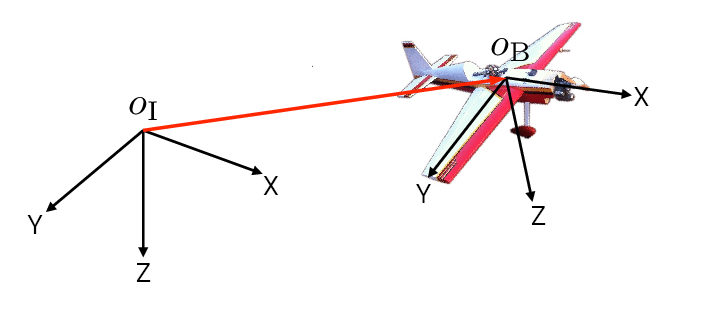
\includegraphics[width=0.7\textwidth]{frames.png}
      	\caption{Definicja układów współrzędnych}
\end{figure}

Korzystając z przedstawionych układów współrzędnych można wyrazić poszczególne elementy wektora stanu układu. W tym miejscu należy zaznaczyć, że w nomenklaturze lotniczej przyjmuje się, że symbol $\bm{y}$ oznacza wektor położenia i orientacji BSP wyrażony w globalnym układzie współrzędnych, a symbol $\bm{x}$ oznacza prędkości kątowe i liniowe wyrażone w układzie współrzędnym związanym z BSP. Oznaczenia te kolidują z oznaczeniami wektora stanu i wyjścia z poprzedniego rozdziału. Od tego miejsca wykorzystana zostanie właśnie ta nomenklatura.\\

Położenie i orientacja BSP zdefiniowana jest jako:
\[
	      		 \bm{y} = \begin{bmatrix}x & y &  z & \varphi & \Theta & \Psi  \end{bmatrix}^{T}_{W} \hspace{10pt} \text{lub} \hspace{10pt} \begin{bmatrix}x & y & z & q_0 &  q_x &  q_y & q_z  \end{bmatrix}^{T}_{W}
\]

gdzie $x, y, z$ to położenie, a orientacja BSP wyrażona jest za pomocą trzech kątów lotniczych $\varphi, \Theta,  \Psi$ lub za pomocą kwaternionu orientacji. Wyrażenie orientacji za pomocą kątów lotniczych pozwala w sposób intuicyjny powiązać kąt z orientacją BSP. Pierwszy z kątów $\varphi$ to kąt przechylenia (ang. roll) tj. kąt przechylenia BSP na skrzydło. Dodatni kąt przechylenia to przechylenie samolotu na prawe skrzydłu. Drugi z kątów $\Theta$ to kąt pochylenia (ang. pitch) tj. kąt pochylania dziobu BSP w górę lub dół. Dodatni kąt pochylenia oznacza dziub zadarty do góry. Ostatni z kątów $\Psi$ opisuje odchylenia (ang. yaw) czyli kąt azymutalny, kierunek kursu. Zerowy kąt odchylenia oznacza skierowanie BSP na północ. Kąt odchylenia może być utożsamiany ze wskazaniem kompasu. Kąty lotnicze zostały dodatkowo przedstawione na rysunku (\ref{RPY}).

\begin{figure}[!h]
   	\centering
      	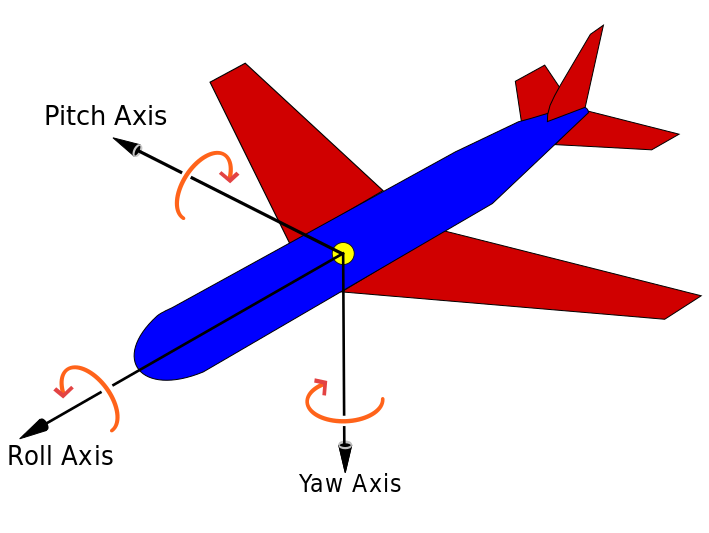
\includegraphics[width=0.5\textwidth]{RPY.png}
      	\caption{Kąty lotnicze}
      	\label{RPY}
\end{figure}

Oprócz przedstawiony zalet opis orientacji przy pomocy kątów lotniczych ma zasadnicze wadę -- niejednoznaczność. Oznacza to, że ta sama orientacja może zostać wyrażona przy pomocy przy pomocy różnych trójek kątów. Jest to szczególnie ważne dla układu sterowania. Orientacja zadana w kątach lotniczych może różnić się od orientacji aktualnej samolotu jedynie konfiguracją. Tym samym układ będzie wykonywał niepotrzebne zmiany orientacji, które finalnie doprowadziłyby go do tego samego stanu. Bardziej ogólnym sposobem wyrażenia orientacji są kwaterniony. Kwaternion w jednoznaczny sposób definiuje orientację, a także pozwala na obrót pomiędzy układami bez konieczności budowania macierzy rotacji. Można pokazać ze kwaternion odpowiada obrotowi oś-kąt.\\

Kolejnym elementem wektora stanu BSP jest wektor prędkości zdefiniowany następująco:
\[
	\bm{x} = \begin{bmatrix}U & V & W &  P & Q & R  \end{bmatrix}^{T}_{B}
 \]
 
 gdzie U, V i W to prędkości liniowe wyrażone zgodne z wektorami układu ruchomego, a P, Q i R to wektor prędkości kątowej zrzutowany na osie układu ruchomego.
 
 Ostatnim elementem wektora stanu BSP jest wektor prędkości kątowych silników:
 \[
	\bm{\omega} = \begin{bmatrix}\omega_1 & \omega_2 & ... &  \omega_{m}  \end{bmatrix}^{T}
 \]
 Rozmiar wektora $\bm{\omega}$ jest zależny od liczby silników \texttt{m} w które został wyposażony BSP. W przypadku silników rotorowych odpowiada on bezpośrednio prędkości wału silnika, w przypadku innych silników jest on jedynie miarą rozpędzenia danego silnika.\\
 
Finalnie wszystkie z przedstawionych wektorów ujęte zostają w zbiorczy wektor stanu układu. zdefiniowany następująco:
\[
      	\begin{bmatrix} \bm{y}\\ \bm{x} \\  \bm{\omega} \end{bmatrix}
\]

Po całościowym zdefiniowaniu wektora stanu układu należy poruszyć temat przyjętych jednostek. W projekcie zostało przyjęte założeniu o wyrażeniu stanu układu przy pomocy jednostek SI (MKS). Położenie wyrażone jest zatem w metrach, do opisu kątów zastosowane zostały radiany. Prędkości liniowe zostały wyrażone w metrach na sekundę, a prędkości kątowe w radianach na sekundę.
Co warto zaznaczyć do wektora stanu mogłyby zostać dodane również inne elementy opisane równaniami różniczkowymi takie jak powierzchnie sterowe, bądź inne elementy mechaniczne. W opracowywanym modelu bezwładność tych elementów została jednak pominięta.

\subsubsection{Model matematyczny BSP}

W poprzednim rozdziale zdefiniowany został stan BSP. W tym rozdziale przedstawione zostanie według jakich praw zmienia się stan układu i co ma na niego wpływ. Zakłada się, że BSP można traktować jako bryłę sztywną, a do zapisania zależności wykorzystane zostaną następujące prawa i twierdzenia:

\begin{enumerate}
\item prędkość jest pochodną położenia,
\item zasada zmienności pędu i krętu, stanowiąca uogólnienie II zasady dynamiki Newtona głosi, że pochodną pędu po czasie jest wypadkowa siła działająca na układ, a pochodną krętu po czasie jest wypadkowy moment działający na układ,
\item silnik można traktować jako człon inercjalny pierwszego rzędu.
\end{enumerate}

Zgodnie z pierwszą zależnością gdyby położenie i prędkość były wyrażone w tym samym układu można by błędnie pomyśleć że $\bm{\dot{y}} = \bm{x}$. Nie jest to jednak prawdą, gdyż prędkość kątowa nie stanowi bezpośrednio pochodnej kątów lotniczych. Niewątpliwe odpowiednich przekształceń wymaga również wyrażenie pochodnej gdy orientacja dana jest jako kwaterniony. Wtedy oprócz odpowiedniej transformaty może pojawić się problem nieunormowania kwaternionu tj. niezachowania jednostkowej normy kwaternionu na skutek kumulujących się błędów arytmetyki komputera. Sposobem zapobiegania temu zjawisku jest np. metoda stabilizowania normy kwaternionu. Mając na uwadze wspominane problemy oraz różne układy w których wyrażone są wektory $\bm{y}$ i $\bm{x}$ można zapisać następującą zależność:
\[
	\bm{\dot{y}} = T(\bm{y}, \bm{x})
\]

Dokładny opis funkcji T zaczerpniety został z publikacji \cite{energies}, a metoda stabilizacji normy kwaternionu z publikacji \cite{quaterion}.\\ %TODO rozwinąc

Pęd bryły sztywnej $\bm{\vec{p}}$ można wyrazić jako:
\[
	\bm{\vec{p}} = m \cdot \bm{\vec{v}}
\]
gdzie $m$ to masa BSP, a $\bm{\vec{v}}$ to wektor jego prędkości liniowych.

Analogicznie kręt (moment pędu) bryły sztywnej $\bm{\vec{L}}$ można wyrazić jako:
\[
	\bm{\vec{L}} = J \cdot \bm{\vec{\omega}}
\]
gdzie $J$ to macierz bezwładności BSP, a $\bm{\vec{\omega}}$ to wektor jego prędkości kątowych. Zgodnie z zasadą zmienności pędu można zapisać następujące zależności:
\[
	\begin{aligned}
	\frac{d\bm{\vec{p}}}{dt} & = \bm{\vec{F}}\\
	\frac{d\bm{\vec{L}}}{dt} & = \bm{\vec{\tau}}
	\end{aligned}
\]
gdzie $\bm{\vec{F}}$ to wypadkowa siła przyłożona do BSP, a $\bm{\vec{\tau}}$ to wypadkowy moment siły działający na BSP. Korzystając z własności rachunku macierzowego powyższe zależności można połączyć uzyskując tym samym zależność:
\[
              \begin{bmatrix}\frac{d\bm{\vec{p}}}{dt}\\ \frac{d\bm{\vec{L}}}{dt} \end{bmatrix} = \begin{bmatrix}\bm{\vec{F}}\\ \bm{\vec{\tau}} \end{bmatrix} = \bm{\vec{f}}
\]
gdzie $\bm{\vec{f}}$ to uogólnione oddziaływanie na układ. Na koniec poprzez policzenie odpowiednich pochodnych (pamiętając o regule pochodnej iloczynu) możliwe jest uproszczenie zapisu do postaci:

\[
	\bm{M} \bm{\dot{x}} +  \bm{\Omega} \left( \bm{x} \right) \bm{M} \bm{x} = \bm{f}
\]
\[
	\bm{\Omega} = \begin{bmatrix}
	0 & -R & Q & 0 & 0 & 0 \\
	R & 0 & -P & 0 & 0 & 0 \\
	-Q & R & 0 & 0 & 0 & 0 \\
	0 & -W & V & 0 & -R & Q \\
	W & 0 & -U & R & 0 & -P \\
	-V & U & 0 & -Q & P & 0 
	\end{bmatrix}
\]
\[
	\bm{M} = \begin{bmatrix}
	m\cdot \bm{ I_{3x3}} & \bm{0_{3x3}} \\ \bm{0_{3x3}} & \bm{J}
	\end{bmatrix}
\]
gdzie $\bm{M}$ jest macierzą masową powstała przez połączenie masy i macierzy bezwładności, a $\bm{\Omega}$ to tzw. macierz żyroskopowa.\\

Ostania z przedstawionych na początku rozdziału zależności dotyczy zachowania silnika. Przyjętym modelem dla silnika elektrycznego jest człon inercyjny pierwszego rzędu. W takim modelu wartość przyśpieszenia kątowego jest zależna od różnicy pomiędzy wartością zadaną, a aktualną. W teorii sterowania różnicę tą nazywa się uchybem. Dodatkowo w modelu występuje współczynnik skalujący nazywany stałą czasową T. Układ równań różniczkowych opisujących zachowanie silnika wyraża się następująco:
 \[
	T \frac{d\omega}{dt} + \omega = \omega_{ZADANA}
\]
gdzie $\omega_{ZADANA}$ to prędkości kątowe zadane przez układ sterowania. Dla zilustrowania zachowania silnika na rysunku (\ref{rotor_step}) przedstawiono wykres prędkości kątowej silnika w funkcji czasu. W chwili początkowej silnikowi zadana została znormalizowana wartość prędkości wynosząca 1. W 5 sekundzie ruchu wartość zadana została zmieniona na 0.5. Należy zwrócić uwagę że stała T ma dokładną interpretację fizyczną i jest to czas po którym spoczywający układ osiągnie 63.5\% wartości zadanej.

\begin{figure}[!h]
   	\centering
      	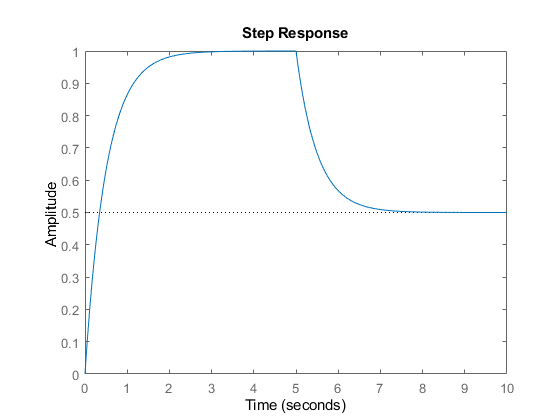
\includegraphics[width=0.5\textwidth]{step.png}
      	\caption{Odpowiedź układu inercyjnego pierwszego rzędu}
      	\label{rotor_step}
\end{figure}






\subsubsection{Siły i momenty działające na BSP}
\subsubsection{Model atmosfery ISA, wiatr}
\subsubsection{Kolizje}
\subsubsection{Odrzut}
\subsubsection{Przenoszenie ładunku}
\subsection{Sterowanie BSP}
\subsubsection{Regulacja i sterowanie}

\subsubsection{System sterowania BSP}
Regulacja i sterowanie, sterowanie w pętli zamkniętej z ujemnym sprzężeniem zwrotnym, model sterowania, drabina pidów
\subsubsection{Regulatory}
PID, LQR, inne.
\subsubsection{System nawigacji}
Czujniki, fuzja pomiarów, Filtr Kalmana

\subsection{Grafika komputerowa}
% Fit the following in the main chapter
%\subsubsection{Procesory graficzne}
%\subsubsection{OpenGL}
%\subsubsection{Potok renderowania}
%\subsubsection{Shadery}
%\subsubsection{Cieniowanie}
%\subsubsection{Model oświetlenia}
\subsubsection{Rysowanie oblamówki modelu za ścianą}
\subsubsection{Ślad po wystrzelonym pocisku}
\subsubsection{Rysowanie liny}
\subsubsection{Wyznaczenie parametrów panelu rotorów}
\subsubsection{Rysowanie radaru}
\subsubsection{Obsługa kontrolerów}

\begin{comment}

Symulacje komputerowe dynamiki ruchu  W szczególności w zagadnieniu jakim jest projektowanie systemów sterowania do bezzałogowych statków powietrznych, zastosowanie takich narzędzi pozwala zminimalizować koszty wytworzenia poprawnie działającego systemu i przyśpieszyć jego rozwój i testowanie.

Celem niniejszej pracy jest opracowanie wirtualnego środowiska do symulacji dynamiki lotu bezzałogowych statków powietrznych. System implementuje podstawowy model dynamiki statków powietrznych wyposażonych w silniki rotorowe, silniki odrzutowe, powierzchnie nośne i powierzchnie sterowe. Pozwala na przeprowadzenie lotu symulowanym obiektem którego parametry określane są przez konfiguracje. System dzieli się na serwer i aplikacje kliencką. Różnorodność modułów pozwala na realizacje rożnych scenariusz (strzał, upuszczenie ładunku, kolizje, wpływ warunków środowiskowych etc.)


\section{Model dynamiki statku powietrznego}

\begin{equation}
\begin{cases}
\dot{Y} =  T(Y) \cdot X + stabilizacja\\ 
A \cdot \dot{X} + \Omega (X) \cdot A \cdot X = F_g + F_a + F_d + F_o
\end{cases}
\end{equation}

gdzie:
\begin{itemize}
\item $Y$ - wektor pozycji i orientacji wyrażony w układzie globalnym
\item $X$ - wektor prędkości postępowej i kątowej w układzie związanym ze statkiem powietrznym
\item $A$ - macierz masowa
\item $\Omega$ - macierz gyroskopowa
\item $F_g$ - siła i moment pochodząca od siły grawitacji wyrażone w układzie związanym ze statkiem powietrznym
\item $F_a$ - siła i moment aerodynamiczny wyrażone w układzie związanym ze statkiem powietrznym
\item $F_d$ - siła i moment zespołów napędowych wyrażone w układzie związanym ze statkiem powietrznym
\item $F_o$ - siła i moment oddziaływań zewnętrznych napędowych wyrażone w układzie związanym ze statkiem powietrznym
\end{itemize}

\begin{equation}
Y = \begin{bmatrix}
x_{NED}\\
y_{NED}\\
z_{NED}\\
q_0\\
q_x\\
q_y\\
q_z
\end{bmatrix}
\end{equation}

\begin{equation}
X = \begin{bmatrix}
\dot{x}_b\\
\dot{y}_b\\
\dot{z}_b\\
P_b\\
Q_b\\
R_b
\end{bmatrix}
\end{equation}

\begin{equation}
F_g = R_{nb}(Y) \cdot  \begin{bmatrix}
0\\
0\\
g
\end{bmatrix}
\end{equation}

\begin{equation}
F_a = \frac{1}{2}\rho \cdot V_{tot}^2 S R_{wb} C_F \\
M_a = \frac{1}{2}\rho \cdot V_{tot}^2 S d R_{wb} C_F
\end{equation}

\end{comment}